\documentclass[a4paper]{article}

\usepackage[utf8]{inputenc}
\usepackage{purev}


\begin{document}
\title{Geometry Pre-test for Summer Program}
\begin{enumerate}
	\item Let $ABC$ be an equilateral triangle and $P$ be a point
		inside the triangle. If the distances from $P$ to the
		three sides are $3$, $5$, and $6$, then find the perimeter
		of the triangle $ABC$.
		\begin{figure}[htpb]
			\centering
			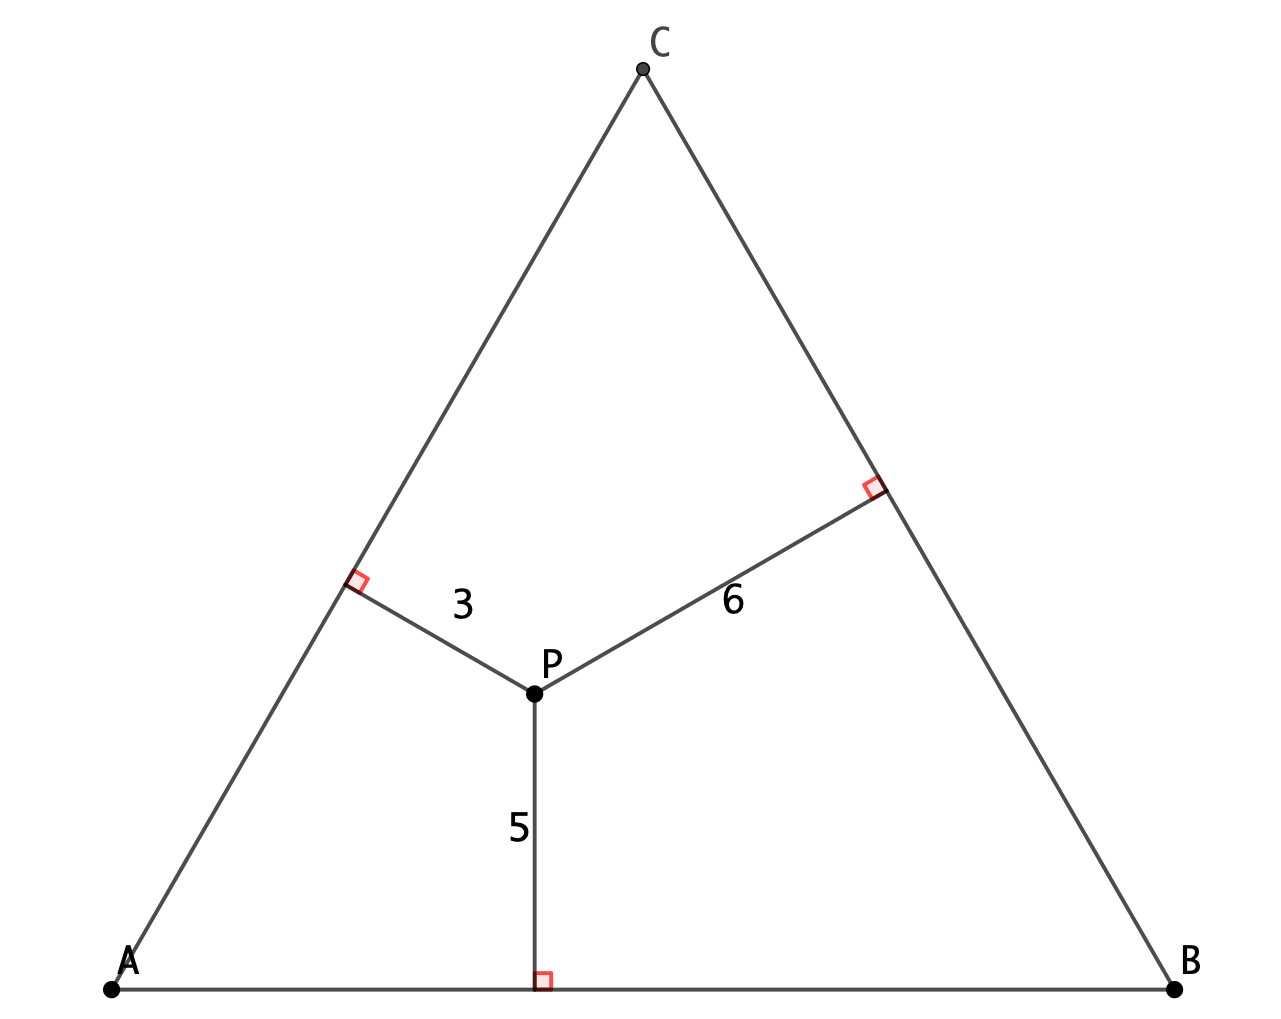
\includegraphics[width=0.5\textwidth]{test_prob1.png}
			\caption{}
			\label{fig:test_prob1-png}
		\end{figure}\\
		\underline{\textbf{Solution}}:\\
		Let $x$ be the length of the side of the equilateral
		triangle $ABC$. We see that the area of $ABC$, 
		\[
			S_{ABC} = \frac{1}{2}x^2\sin60^{\circ} = \frac{x^2\sqrt{3}}{4}
		.\] \\
		On the other hand, the area of $ABC$ is the sum of the
		areas of $APB$, $BPC$, and $CPA$, i.e.
		\begin{align*}
			S_{ABC} &= S_{APB} + S_{BPC} + S_{CPA} \\
			&= \frac{3\cdot x}{2} + 
			\frac{6\cdot x}{2} +
			\frac{5\cdot x}{2}\\
			&= 7x 
		\end{align*}
		Therefore, 
		\[
			\frac{x^2\sqrt{3} }{4} = 7x \implies
			x = \frac{28}{\sqrt{3} }
		.\] \\
		So, the perimeter of the triangle is
		\[
		P_{ABC} = 3\cdot x = 28\sqrt{3} 
		.\] 

		\newpage
	\item Let $ABCD$ be a cyclic quadrilateral, i.e. the points
		$A$, $B$, $C$, and $D$ lie on a same circle, and
		$P$ be the intersection of diagonals $AC$ and $BD$. 
		Given that $AB = 20$, $BC = 2\sqrt{22}$, $CD = 5$, 
		$DA = 6\sqrt{22}$, and $DP = 6$, find the lengths of 
		$AP$ and $CP$.
		\begin{figure}[htpb]
			\centering
			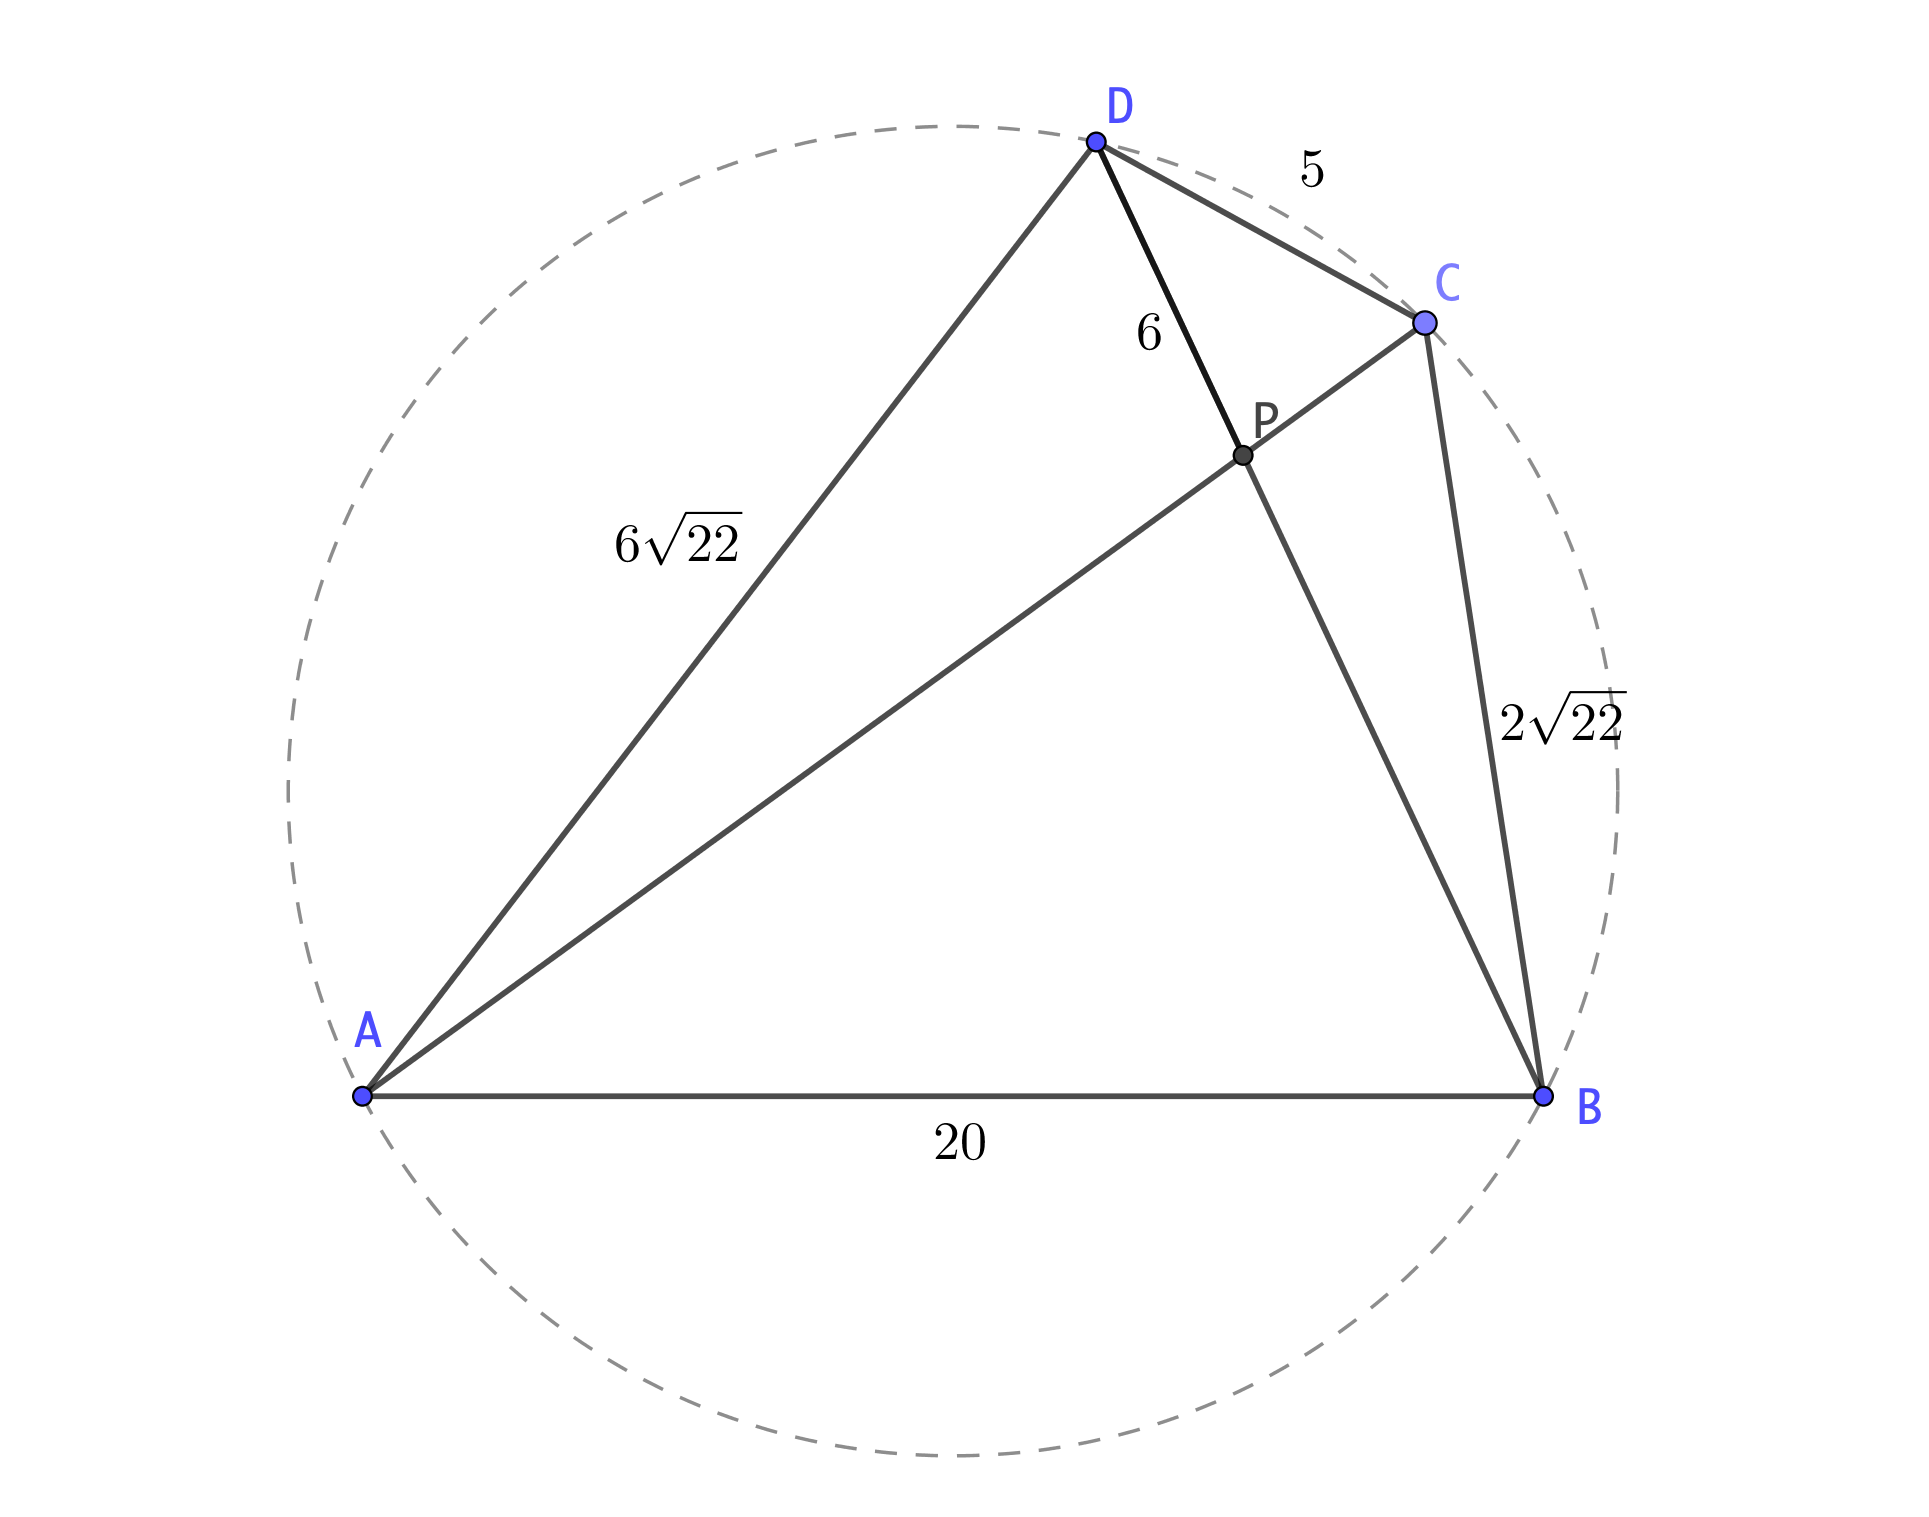
\includegraphics[width=0.5\textwidth]{test_prob2.png}
			\caption{}
			\label{fig:test_prob2-png}
		\end{figure}\\
		\underline{\textbf{Solution}}:\\
		By the property of cyclic quadrilateral, we know that
		\[
		\angle PAB = \angle CAB = \angle CDB = \angle PDC
		.\] 
		Similarly, we see that 
		\[
		\angle PBA = \angle DBA = \angle DCA = \angle DCP
		.\] 
		Therefore, the trianles $PAB$ and $PDC$ are similar. So
		\[
		\frac{AB}{DC} = \frac{PA}{PD} \implies PA = 24
		.\] 
		Now, we also observe that the triangles $PDA$ and $PCB$
		are similar. Hence,
		\[
		\frac{DA}{CB} = \frac{PD}{PC} \implies PC = 2
		.\] 
		\newpage
	\item Let $ABC$ be a right triangle with $\angle ACB = 90^\circ$
		and $P$, $Q$, and $R$ be the midpoints of the sides
		$AB$, $BC$, and $CA$, respectively. Two equilateral 
		triangles $AMR$ and $BQN$ are constructed outside
		of triangle $ABC$. Find $\angle PMN$.
		\begin{figure}[htpb]
			\centering
			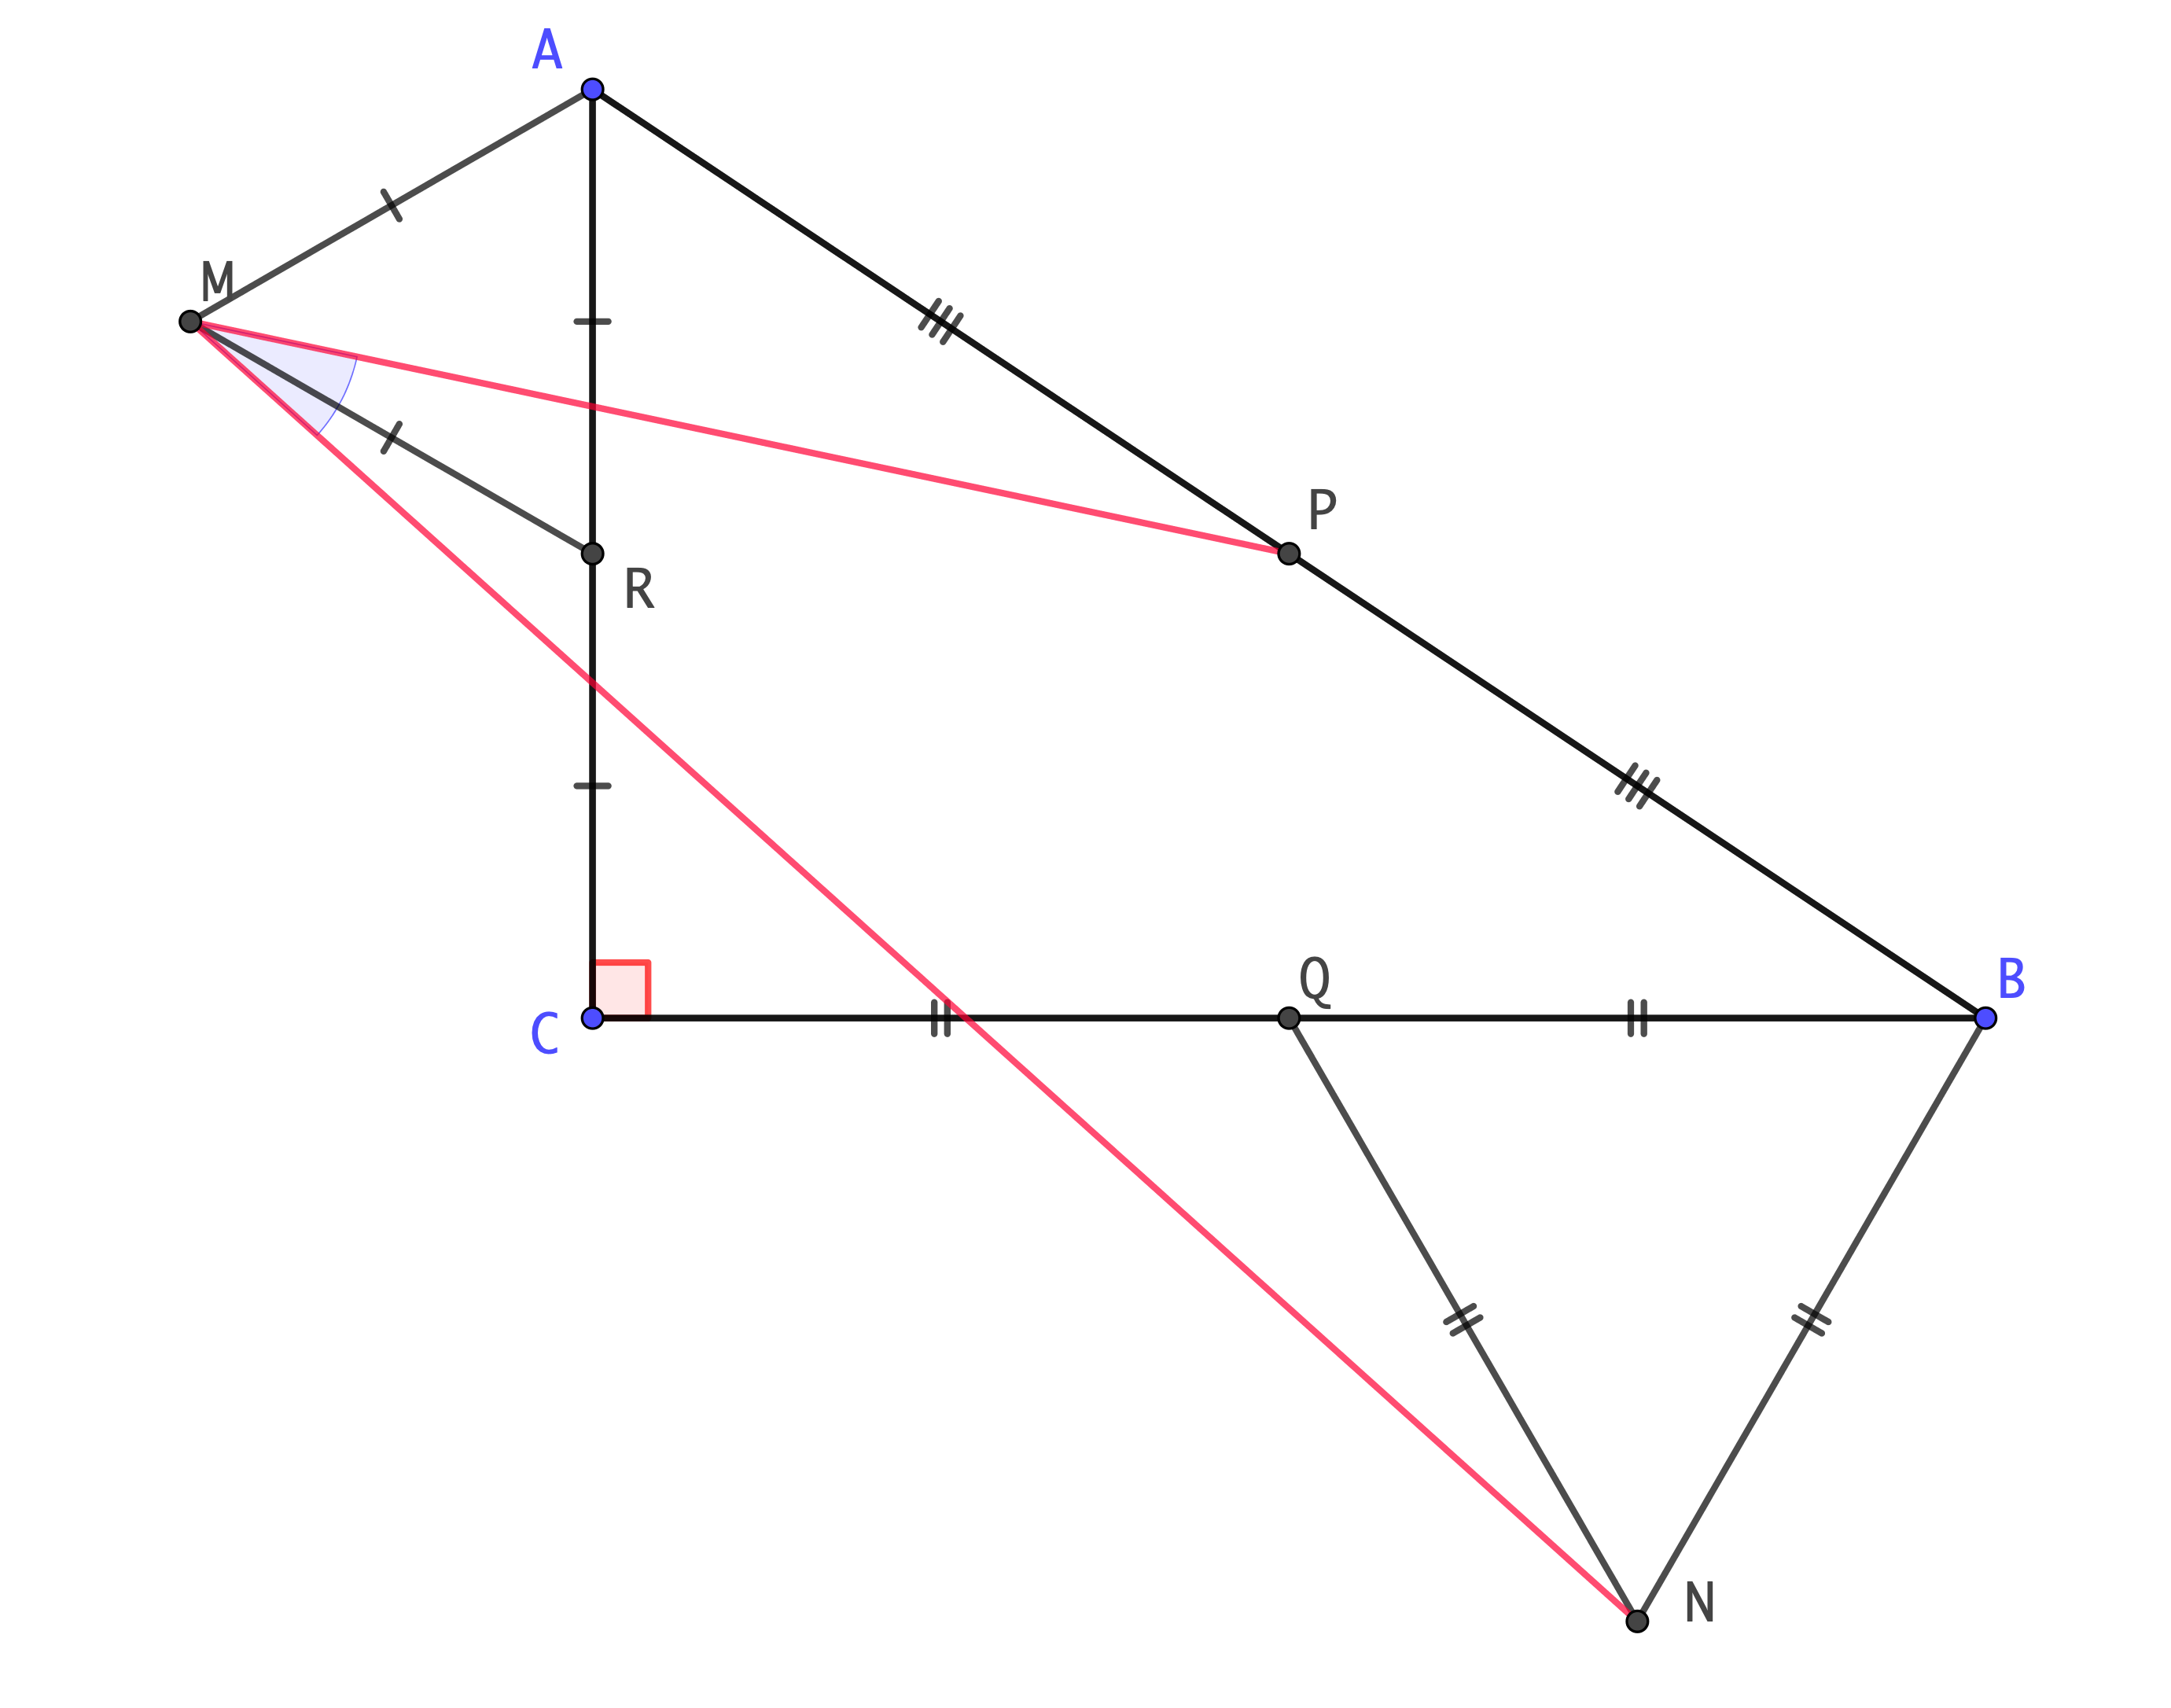
\includegraphics[width=0.5\textwidth]{test_prob3.png}
			\caption{}
			\label{fig:test_prob3-png}
		\end{figure}\\
		\underline{\textbf{Solution:}}\\
		The triangles $MRP$ and $PQN$ are equivalent since
		\begin{itemize}
			\item $MR = AR = \frac{1}{2} AC = PQ$ $\implies$ $MR = PQ$.
			\item $\angle MRP = \angle MRA + \angle ARP = 150^\circ
				= \angle PQB + \angle BQN = \angle PQN$ $\implies$ $\angle MRP = PQN$.
			\item $RP = \frac{1}{2}CB = QB = QN$ $\implies$ $RP = QN$.
		\end{itemize}
		Therefore, $MP = PN$ and $\angle PMR = \angle NPQ$.
		Also, 
		\begin{align*}
			\angle MPN &= \angle MPR + \angle RPQ + \angle QPN\\
			&= \angle MPR + 90^\circ + \angle PMR \\
			&= 90^\circ + (\angle MPR + \angle PMR) \\
			&= 90^\circ + (180^\circ - \angle MRP) \\
			&= 90^\circ + (180^\circ - 150^\circ) \\
			&= 120^\circ
		.\end{align*}
		Since we have found that $MP = PN$, the triangle $MPN$
		is isosceles with $MPN = 120^\circ$. So,  
		\begin{align*}
			\angle PMN &= \frac{1}{2}(180^\circ - \angle MPN)\\
				   &=  \frac{1}{2}(180^\circ - 120^\circ) \\
				   &= 30^\circ
		.\end{align*}
\end{enumerate}
\end{document}
